\cotefile{162-1}
\scanpage{3}

% Upper entries and printed letterhead positioned together to retain the branching callout.
\figure{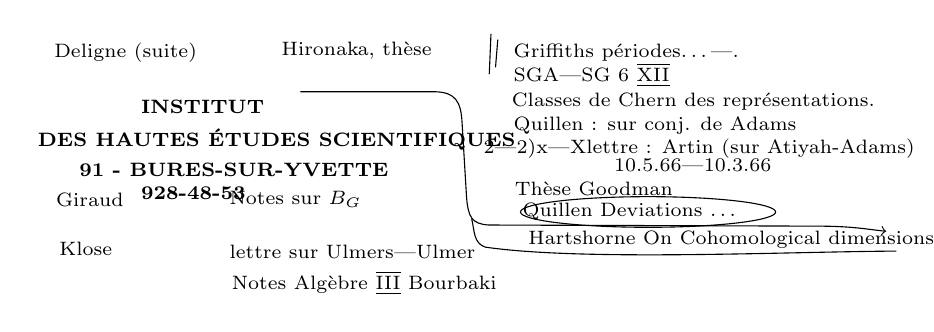
\begin{tikzpicture}[x=.0072cm,y=-.0072cm,every node/.style={anchor=base west,inner sep=0pt,font=\scriptsize}]
\path[use as bounding box] (120,18) rectangle (1668,505);
\node at (166,70) {\deleted{\uline{Deligne} (suite)}};
\node at (567,67) {\deleted{\unsure{Hironaka}, thèse}};
\draw (937,29)--(934,100) (949,39)--(945,88);
\node at (976,70) {\deleted{\unsure{Griffiths} \unsure{périodes}\unsure{\ldots|.}}};
\node at (976,113) {\deleted{\unsure{SGA|SG} 6 $\overline{\underline{\mathrm{XII}}}$}};
\node at (973,157) {\deleted{Classes de Chern des représentations.}};
\node at (976,199) {\deleted{Quillen : sur \unsure{conj.} de Adams}};
\node at (923,240) {\deleted{\unsure{2|2)}\deleted{\unsure{x|X}}\unsure{lettre} : Artin (sur Atiyah-Adams)}};
\node at (1153,271) {\inserted{\deleted{\unsure{10.5.66|10.3.66}}}};
\node at (978,314) {\deleted{Thèse \uline{Goodman}}};
\node at (992,351) {\deleted{Quillen Deviations \ldots}};
\draw (1214,343) ellipse [x radius=225,y radius=27];
\node at (1002,401) {\deleted{Hartshorne On Cohomological dimensions..}};
% The upper branch has an arrowhead; the lower branch runs below the Hartshorne entry.
\draw[->] (601,131)--(839,131) .. controls (874,132) and (884,148) .. (886,185)
 --(894,318) .. controls (897,352) and (903,364) .. (933,366)
 --(1513,368) .. controls (1577,368) and (1602,374) .. (1634,377);
\draw (903,355) .. controls (908,376) and (906,398) .. (927,405)
 .. controls (1100,430) and (1460,413) .. (1652,412);
% letterhead
\node[font=\scriptsize\bfseries] at (319,169) {INSTITUT};
\node[font=\scriptsize\bfseries] at (137,228) {DES HAUTES ÉTUDES SCIENTIFIQUES};
\node[font=\scriptsize\bfseries] at (210,280) {91 - BURES-SUR-YVETTE};
\node[font=\scriptsize\bfseries] at (319,321) {928-48-53};
\node at (169,333) {\deleted{\uline{Giraud}}};
\node at (475,330) {\deleted{Notes sur $B_G$}};
\node at (175,420) {\deleted{\uline{Klose}}};
\node at (475,425) {\deleted{lettre sur \unsure{Ulmers|Ulmer}}};
\node at (479,480) {\deleted{Notes Algèbre $\overline{\underline{\mathrm{III}}}$ Bourbaki}};
\end{tikzpicture}}

\uline{Shih}\quad 1\qquad Rapport à Bourbaki calcul différentiel

\deleted{\uline{3} articles Schwarzenberger sur fibrés vectoriels}

Résumé PTT Grenoble

\deleted{\uline{\unsure{N|M}\illegible{1}}}\qquad \deleted{\unsure{PTTM|PTT M}}

\uuline{Papiers Atiyah} \uline{topologie} et \uline{op. elliptiques}

\deleted{\uline{Bertin}\qquad EGA $\overline{\underline{\mathrm{IV}}}$ \unsure{16--19|16 19} photocopies}

\deleted{\unsure{Mme|Mne} \uline{\unsure{Hakim}}\qquad Séminaire Gabriel deux schémas, Exp $7$}

\uline{Ferrand}\quad 1\qquad \deleted{EGA $\overline{\underline{\mathrm{IV}}}$ 20,21 \deleted{\unsure{photocopies}} épreuves}

Lettre : Dieudonné sur par.factoriel en dim 2

\tikz[baseline=(rr.base)]{\node[inner sep=2pt] (rr) {\deleted{Notes sur R.R.}};\draw (rr.center) ellipse [x radius=3.1em,y radius=.74em];}\ ?

Notes sur le foncteur dét. / \uline{sur cat. de Picard} .

\uline{Jouanolou}\quad 1\qquad \inserted{Papiers Hartshorne (dim. \unsure{ch.|coh.}) et Goodman}

\deleted{Notes cohomologie $\unsure{\ell|l}$-adique}

Papier Hirzebruch (Congrès d'Amsterdam ?) )

\noindent Lettre : Serre $\left\{\begin{array}{l}\text{\unsure{équ.} fonctionnelle \unsure{fonction|fonctions} }L\\ \text{suite, début de monodromie \unsure{....|\ldots}}\end{array}\right.$

\deleted{\uline{Berthelot}\qquad Notes sur stratifications}

\margin{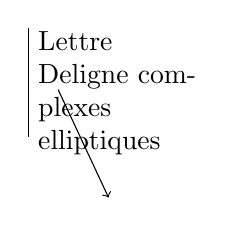
\begin{tikzpicture}[x=1cm,y=1cm,baseline=(md.north)]
\node[anchor=north west,inner sep=0pt,text width=2.05cm,align=left] (md) at (.12,0) {\deleted{Lettre Deligne \unsure{complexes}}\\\deleted{elliptiques}};
\draw (0,.03)--(0,-1.35);
\draw[->] (.38,-.75)--(1.02,-2.12);
\end{tikzpicture}}
% The diagonal marginal arrow descends toward the right edge of the lower cancelled group; no specific textual insertion is inferred.

\deleted{Notes RR (copie de Serre)}

\deleted{Notes Serre sur ${\unsure{\mathrm{ch}|\mathrm{dh}}}^{\unsure{n-i|n-1|n-\nu}}=0$}

\deleted{Calcul $K\unsure{(\mathrm{P}^{n}|\mathrm{CP}^{n}}(\unsure{\overline{\mathrm L}|\mathrm L^{-}|\overline{\mathrm C}}))$}

\deleted{Rapport Serre représentations de groupes finis}

\deleted{\uline{Kleiman}\qquad \unsure{photocopies|Photocopies} EGA $\overline{\underline{\mathrm{IV}}}$ 20}

\deleted{EGA $\overline{\underline{\mathrm{V}}}$}

\deleted{Notes Chev. sur \unsure{grassmanniennes|grassmaniennes}}

\deleted{Note \unsure{Agison|Agišon} \unsure{bidéterminants|holodéterminants}}

\deleted{Problèmes de Géométrie Algébrique}

\deleted{\uline{Verdier}\qquad \unsure{SGAA|SGA 4} fasc. 1, mon exemplaire personnel}

\deleted{\unsure{Gabriel}}

\deleted{\uline{\unsure{Terjanian|Terzanian}}\qquad \unsure{Articles|Article} Greenberg sur \unsure{$C_i$|$C_1$}}

% archive sheet number: 2

\clearpage
